\newif\iflettablesappear
  \lettablesappearfalse    % Tables disappear
% \lettablesappeartrue     % Tables appear;  but what other errors are there?


\newif\ifsinglecolumn
% <-------------------------------------------------------------------------------
%\singlecolumntrue        % single column 
\singlecolumnfalse       % double column 

\newif\ifpeerreview   
%\peerreviewfalse         % final 
 \peerreviewtrue          % anonymized      

\newif\iftogether
%\togethertrue            % Figures 5 and 6 together
\togetherfalse           % Figures 5 and 6 not together


\newif\iftogethersa
%\togethersatrue          % Figures 7 and 8 together
\togethersafalse         % Figures 7 and 8 not together

\newif\iffigninewide
% \figninewidefalse         % Figure 9  Don't ever use
\figninewidetrue          % Figure 9    

% The final version
\ifpeerreview
\documentclass[preprint,3p,times,twocolumn]{elsarticle}  %  peer review
\else
\documentclass[final,3p,times,twocolumn]{elsarticle}  % onecolumn
\fi
%\documentclass[10pt,conference,a4paper,twocolumn, draft] {IEEEtran} % Draft
\usepackage{lipsum}
\usepackage{kantlipsum}
\usepackage[switch]{lineno} % remove 'draft', insert \linenumbers just after \begin{document}
\usepackage{graphicx}
\usepackage{epic}
\usepackage{figsize}
\usepackage{float}
\usepackage{hyperref}
\usepackage[section]{placeins}
\usepackage{cite}
\usepackage{amsmath}
\usepackage{amssymb}
\usepackage{amsfonts}
\usepackage{bm}
\usepackage{flushend} % ends article with equal column length
\usepackage{verbatim} % for commenting out rubbish
\usepackage{enumitem} % for small roman letter enumerate: 
                      %\begin{enumerate}[label=\roman*]
                      % but avoid 
                      %\begin{enumerate}[label=(\roman*).]
\usepackage{booktabs} % for decent looking tables
\usepackage{tabularx,ragged2e} % For RaggedRight 
\usepackage{multirow} % for multirow
\usepackage{geometry}
\usepackage{longtable} % for longtable
%%%%%%%%%%%%%%%%%%%%%%%%%\usepackage{caption}   % For caption
\usepackage[font=small,labelfont=bf,margin=\parindent,tableposition=bottom]{caption}
\usepackage{xcolor}   % For color


%   \usepackage{ulem} %For striking out text    %% Cannot use with latexdiff


\hyphenation{im-ple-men-ta-tion}
\newcommand{\best}[1]{{\bf\textcolor{blue}{#1}}}
\newcommand{\bestt}[1]{{\bf\textcolor{blue}{#1}}}

\graphicspath{{figures/}}

\journal{Heliyon}
\begin{document}
\begin{frontmatter}
\title{This Article Shows that \texttt{elsarticle.cls} Does not Work Properly}
\ifpeerreview
\author{Reg Dodds\corref{corrauth}}
\ead{rdodds@uwc.ac.za}
\address{Department of Computer Science, University of the Western Cape, South Africa}
\else
\author{Reg Dodds\corref{corrauth}}
\ead{rdodds@uwc.ac.za}
\address{Department of Computer Science, University of the Western Cape, South Africa}
\fi
\cortext[corrauth]{Corresponding author}

\begin{abstract}
We recently submitted a paper to Helyion, that, admittedly still needed 
a lot of work, without checking the output produced by their \texttt{elsarticle.cls}
 style sheet.  The editor summarily threw our paper out because it had 
missing references, e.g. \ldots\ Table~\ref{table:1} and~\ref{table:2}. 
 What was more upsetting than the rejection of the paper, was that two tables 
were arbitrarily omitted as is shown in this paper.  By adding some lines 
or removing them, the tables appear or disappear as if by magic.  

Adding \verb!\linenumbers! or leaving it out does help.

Using \verb!final! or \verb!preprint! does not affect the misbehaviour.

Clearly, \verb!elsarticle.cls! does not function correctly.

\lipsum[1]
\end{abstract}
\begin{keyword}
Deep learning algorithm \sep sequential models \sep metrics \sep
optimisation techniques \sep large datasets \sep validation
\end{keyword}
\end{frontmatter}
%   \twocolumn
\linenumbers
%--------------------------------------------------------------------------------------
% selfisa_framework.tex
\section{Introduction}\label{sec:intro}
\begin{figure*}%[!htp]
%
\centering
\centering{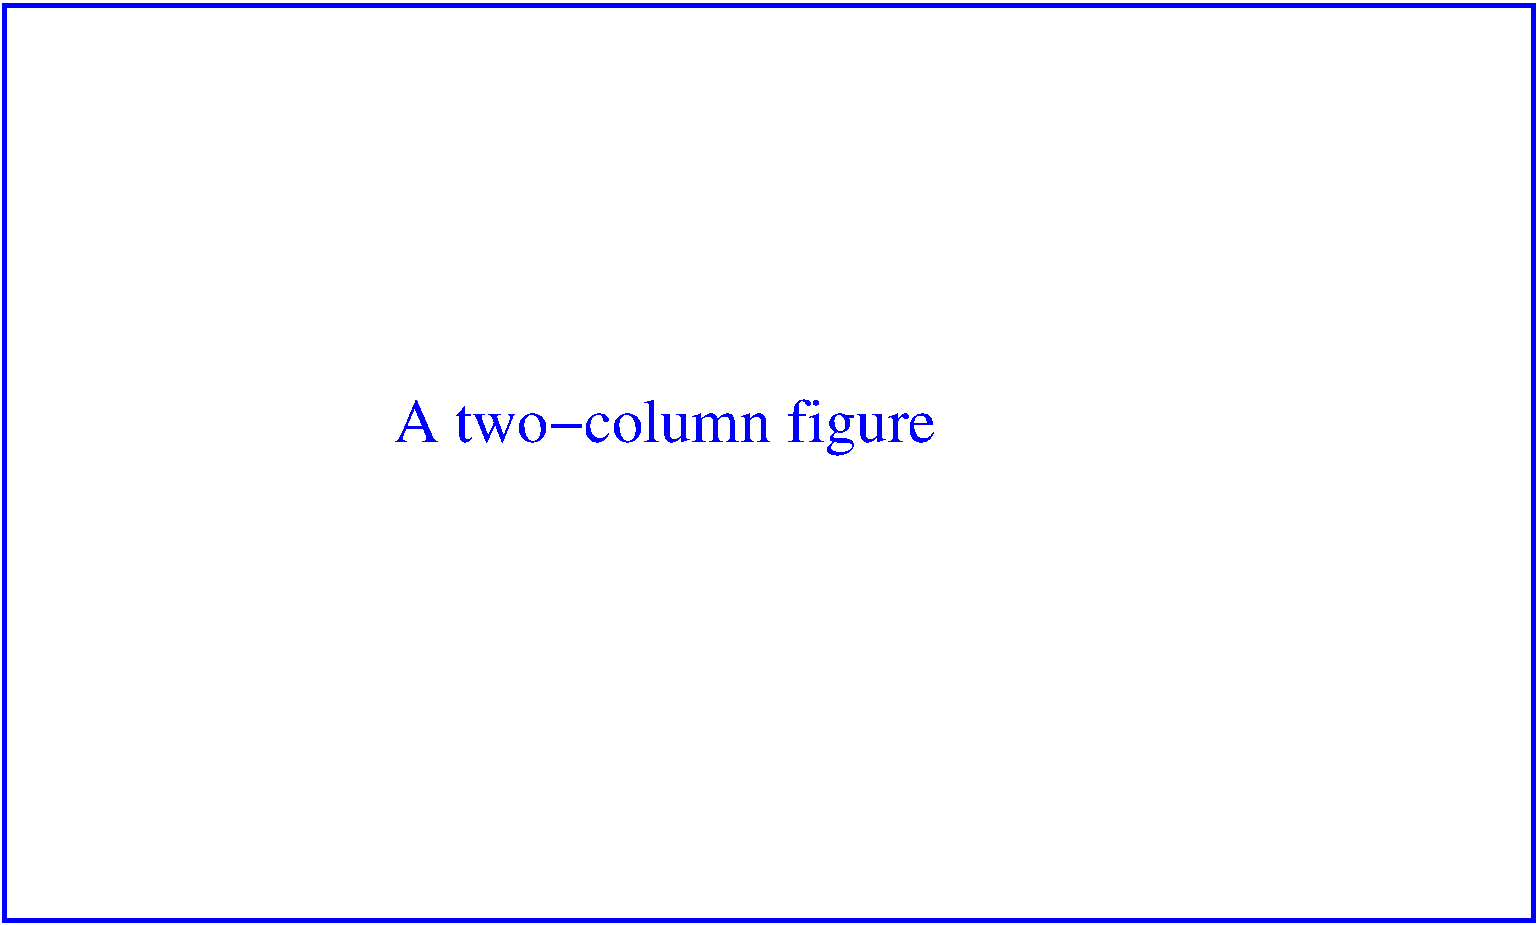
\includegraphics[bb=010 010 770 436,height=200pt,width= 450pt]{figure1.pdf}}
\caption{Quisque ullamcorper placerat ipsum}\label{fig:1}
\end{figure*}
\lipsum[3-5]
\section{Aliquam dolor odio}\label{sec:methods}\label{sec:implementation}\label{sec:finalresults}\label{section:discussion}\label{section:conclusion}\label{sec:acknowledgment}\label{section:annexures}

Curabitur et nunc. Aliquam dolor odio, com- modo pretium, ultricies non,
 pharetra in, velit. Integer arcu est, nonummy in, fermentum faucibus, egestas 
vel, odio.

\subsection{Nulla malesuada porttitor diam}\label{subsec:sf1}% Step 1
Nulla malesuada porttitor diam. Donec felis erat, congue non, volutpat at,
 tincidunt tristique, libero. Vivamus viverra fermentum felis. Donec nonummy 
pellentesque ante. Phasellus adipiscing semper elit. Proin fermentum massa 
ac quam. Sed diam turpis, molestie vitae, placerat a, molestie nec, leo.
 Maecenas lacinia.  

\subsection{Nulla malesuada porttitor diam.}\label{subsec:sf2}
\lipsum[3-3]

\subsection{Implement best performing models}\label{subsec:sf3} 
\lipsum[4-5]
  
\subsection{Suspendisse vel felis.}\label{subsec:sf4}
Suspendisse vel felis. Ut lorem lorem, interdum eu,
tincidunt sit amet, laoreet vitae, arcu. Aenean faucibus
pede eu ante. Praesent enim elit, rutrum at, molestie
non, nonummy vel, nisl. Ut lectus eros, malesuada sit
amet, fermentum eu, sodales cursus, magna. Donec eu
purus. Quisque vehicula, urna sed ultricies auctor, pede
lorem egestas dui, et convallis elit erat sed nulla. Donec
luctus. Curabitur et nunc. Aliquam dolor odio, com-
modo pretium, ultricies non, pharetra in, velit. Integer
arcu est, nonummy in, fermentum faucibus, egestas vel,
odio.

\subsection{Pellentesque habitant morbi tristique senectus}\label{subsec:sf5}% Step 5
Pellentesque habitant morbi tristique senectus et netus et malesuada fames 
ac turpis egestas. Donec odio elit, dictum in, hendrerit sit amet, egestas 
sed, leo. Prae- sent feugiat sapien aliquet odio. Integer vitae justo. Aliquam 
vestibulum fringilla lorem. Sed neque lectus, con- sectetuer at, consectetuer 
sed, eleifend ac, lectus. Nulla facilisi. Pellentesque eget lectus. Proin 
eu metus. Sed porttitor. In hac habitasse platea dictumst. Suspendisse eu 
lectus. Ut mi mi, lacinia sit amet, placerat et, mollis vitae, dui. Sed 
ante tellus, tristique ut, iaculis eu, male- suada ac, dui. Mauris nibh 
leo, facilisis non, adipiscing quis, ultrices a, dui.  Morbi luctus, wisi 
viverra faucibus pretium, nibh est placerat odio, nec commodo wisi enim 
eget quam.  
\begin{equation}\label{eq:1}
           N_h    =       \frac{\alpha N_s}
%                       ------------------ 
                            {N_i+ N_o},
\end{equation}
Quisque libero justo, consectetuer a, feugiat vitae, port- titor 
eu, libero. Suspendisse sed mauris vitae elit sollic- itudin malesuada. 
Maecenas ultricies eros sit amet ante.  Ut venenatis velit. Maecenas sed 
mi eget dui varius euismod. 


%laoreet varius, eros tellus scelerisque quam, pel- lentesque hendrerit 
%ipsum dolor sed augue. Nulla nec lacus.  Suspendisse vitae elit. Aliquam 
%arcu neque, ornare in, ullamcorper quis, commodo eu, libero. Fusce sagittis 
%
%         PLAY WITH THESE LINES
%
%erat at erat tristique mollis. Maecenas sapien libero, molestie et, lobortis 
%in, sodales eget, dui. Morbi ultrices rutrum lorem. Nam elementum 
%ullamcorper leo. Morbi dui. Aliquam sagittis. Nunc placerat. Pellentesque 
%tristique sodales est. Maecenas imperdiet lacinia velit. Cras non urna.
% Morbi eros pede, suscipit ac, varius vel, eges- tas non, eros. Praesent 
%malesuada, diam id pretium elementum, eros sem dictum tortor, vel consectetuer 
%odio sem sed wisi.

\subsection{Phasellus aliquet volutpat odio.}\label{subsec:sf6}% Step 6   
Phasellus aliquet volutpat odio. Vestibulum 
ante ipsum primis in faucibus orci luctus et ultrices po- suere cubilia 
Curae; Pellentesque sit amet pede ac sem eleifend consectetuer. Nullam elementum,
 urna vel im- perdiet sodales, elit ipsum pharetra ligula, ac pretium ante 
justo a nulla. Curabitur tristique arcu eu metus.  Vestibulum lectus. 

\section{Vestibulum lectus}\label{sec:implementation}\label{section:results}
Phasellus aliquet volutpat odio. Vestibulum ante ipsum primis in faucibus 
orci luctus et ultrices po- suere cubilia
Figure~\ref{fig:1} in Section~\ref{sec:methods}.
Curabitur tristique arcu eu metus.  Vestibulum lectus. 

\subsection{Aenean nonummy magna non leo}
Nulla in ipsum. Praesent eros nulla, congue vitae,
euismod ut, commodo a, wisi.~\citep{probst19} Pellentesque habitant
morbi tristique senectus et netus et malesuada fames ac
turpis egestas. Aenean nonummy magna non leo.

\subsection{Nulla malesuada porttitor diam.}
%\item % Step 2---
Nulla malesuada porttitor diam. Donec felis erat, congue non, volutpat at,
 tincidunt tristique, libero~\citep{chang18}, vivamus viverra fermentum felis. Donec nonummy 
pel- lentesque ante. Phasellus adipiscing semper elit. Proin fermentum massa 
ac quam. Sed diam turpis, molestie vitae, placerat a, molestie nec, leo.
 Maecenas lacinia.  Nam ipsum ligula, eleifend at, accumsan nec, suscipit 
a, ipsum. Morbi blandit ligula feugiat magna. Nunc eleifend consequat lorem.
 Sed lacinia nulla vitae enim.  Pellentesque tincidunt purus vel magna. 
Integer non enim. Praesent euismod nunc eu purus. Donec bibendum quam in 
tellus. Nullam cursus pulvinar lectus in~\ref{section:B}.  

Duodecim analysi sequentiae algorithm et exempla a litteris recensitis notata sunt
and used as candidatus artificia faciendo. Haec exempla variis coniunctionibus utuntur
gatum recurrens neural ligula,
autoencoders, retiacula convolutionis neuralis, machinationes bidirectiones, attention
mechanismi, artificia ensemble, et alta et vanilla architecturae. The
horum exempla subtiliter predictive iudicium criteriis perpensum est
et metri e litteris recognitis. Sed aliquam
auctores metri qualitivi usi, et metri consuetudine facta construebantur
bisce lunt quantitare. Criteria comprehendit: (1) perficiendi
accurate per medium errorem absolutum (MAE), medium erroris quadrati (MSE) et
$R^2$ determinationis coefficiens; (2) constantia; (3) efficientiam; (IV) explainientis;
et (5) iterationes aestimatae. Consilium altae doctrinae algorithmae
per rubricans involvit automatic configurationem trainable / discibilis
et parametri non-trainable. Hi ambitum numerum commovent
laminis in architectonica. Numerus parametri metiri
ut cumulativo numero nexuum inter ordines eorumque
respective biases~\citep{probst19}. Morbi sunt
mathematici metrici qui pervestigationes praebent circa exemplar profunditatem,
 capacitatem et multiplicitatem quae significantes vim habent in altiore 
observantia exemplaris. In hac investigatione, it magni momenti fuit ut 
metrica illa demonstrarent accurationem, constantiam et efficientiam exemplorum 
quantum ad ambitum parametri statutum totum tempus suscipit ut certa disciplina 
dataset instituendi. Hoc provisum per viam quantitare deviationis inter 
praedicta et ipsa bona et diversis exemplaribus agendi rationem architecturae 
ordinare multiplicitas. 

\lipsum[31-31]
%  Removing the \% makes the elsarticle style sheet work.
~\citep{sengupta96} et~\citep{hossin15}; 

%\lipsum[42-42]---
Metrica illa demonstrarent accurationem, constantiam et efficientiam exemplorum 
quantum ad ambitum parametri statutum totum tempus suscipit ut certa disciplina 
dataset instituendi. Hoc provisum per viam quantitare deviationis inter 
%praedicta et ipsa bona et diversis exemplaribus agendi rationem architecturae 
temere variationes ad cujusvis exemplar perficiendum, ejus facultatem afficiens
ut accurate praedicere mores alicujus dataset. nativus iudicium
metrice---in his variationibus incertis fundatum est patietur comparatio cum
classica metrica existentium. Et ideo metri metiri debent
constantia---seu stabilitas---et efficaciam ad exemplar, refertur
ad instar BonBONUM constantia et BonBONUM efficientia respective, definiuntur
in 2 et 3. In hoc opere, inferioris BonBONUM constantia valoris
altiorem BonBONUM efficientiam output emendationem indicant.

BonBONUM in duabus notis nummariis notatis explicatum est. A constituebant 
constantiam quae metrica appellatur exemplar constantiae \textit{BonBONUM}
 definitum praebere modum constantiae exemplar expositum ad sequentia discreta 
irregularia; et datum est per Equationis (\ref{eq:2}).
\begin{equation}\label{eq:2}
                   S\!{_s} = \frac{\alpha|m_1-m_2|}
%                         --------------------
                               {m_1+m_2},
\end{equation}
ubi $S\!{_s}$ est \textit{BonBONUM exemplar consistens}, $m_1$ est 
MAE exemplari par GBP/BTC data, $m_2$ est MAE exemplari par JPY/BTC data 
et $\alpha = 2$ est pondus fere $m_1$ et $m_2$. 

Haec metrica differentiam MAE inter exempla dat normalized. inferiora
values de $S_s$ indicant melius perficientur constantia.

Similiter, consuetudo disposita efficientia metrica quae vocatur \textit{BonBONUM
exemplar efficientiae} definiebatur in ordine ad quantitare et comparare
efficacia exemplorum fub comparatione. Haec metrica computationes
numerus ratio parametri et exemplare trainable
tempus instituendi exemplar; valorem metricum altius eo citius
exemplar cum dato numero parametrorum tractabilium instituere potest.
Notandum tamen est architecturae algorithmus effectum habere significantem
in hac regula cum numerus parametri connectuntur
architecturae. 
\begin{equation}\label{eq:3}
                   E_s= \frac nt,
\end{equation}
ubi $E_s$ est \textit{BonBONUM exemplar efficiens}, $n$  est numer
parameteres et $t$ est tempus disciplini in secundi. 

Exemplum, duo exempla dantur cum totidem parametris trabibilibus;
sed primo agmine trabi- bilis est in dimidio temporis tantum secundo ;
valorem primi exemplar in $E_s$ erit duplo altitudine
secundo, ostendens quod duplo velocius totidem parametri.
In secundo exemplo, duo exempla dantur in eadem disciplina temporis, sed
cum duplici numero parametri ut exemplar primo
secundum, valorem primi exemplaris $E_s$ erit duplex secundi;
significans numerum duplicem parametri for . instituere posse
eadem disciplina est. Omnes-in omnibus, maiorem valorem of $E_s$ maiorem indicat
exercendi dexteritas. 

\subsection{Exsequendam optima faciendo exempla }
%\item % Step 3---
Exsecutio candidatorum architecturae selectarum, algorithmorum
et exempla cum selectis discretis irregularibus seriebus: Hoc factum est utens idem
processus in iuxta loce, data, algorithmae et criteriis aestimatio
Gradus 1 et 2. Summa 30 variabilium cum supra 410 sub variabilium
  reperiuntur et describuntur in~\ref{sec:B}. Vide GitHub ad codicem. 

Exempla ad hunc gradum disposita quattuor architecturae innituntur: (1).
GRU, (2) LSTM, (3) Bi et (4) auto-attentionis mechanismi architecturae. Haec
eximie bene discreta irregularia sequentia.

  Omnium exemplorum eventus compendiantur in Tabula~\ref{table:3} et
singula in promptuario GitHub in quibus omnia ex codice usus est ad producendum
hi proventus in sectione ~\ref{section:annexures} caventur. Maxime de
exempla --- quae in gradibus 1 et 2 --- producuntur praedictiones quae passi sunt
de solidis verticalibus et horizontalibus obsessio a terra veritas
valores in figuris illustrati~\ref{fig:2} et~\ref{fig:3}. A verticale
obsessio habet effectum quantitatis in predictis, i.e. exactum valorem
praedictum erit aliud ad terram veritatem, dum a
trabea horizontalis praesentiam praedictionis mora indicat. In data
%puncta magnis inflexionibus in pretio, horizontalibus vices faciunt errores
%directio praedictionis. Praedicens exemplar, quod est capax
%talis appellandi quaestio ea est quae facultatem servandi habet
%eadem magnitudine verticali. % , sed transferre ad dimensionem horizontalem
% perspicientiam providere futuras inclinatiae antequam fiant. 

Nullam eleifend justo in nisl. In hac habitasse platea dictumst. Morbi nonummy.
 Aliquam ut felis. In velit leo, dictum vitae, posuere id, vulputate nec,
 ante. Maecenas vitae pede nec dui dignissim suscipit. %Morbi magna. Vestibulum 
%id purus eget velit laoreet laoreet.  Praesent sed leo vel nibh convallis 
%blandit.% Ut rutrum.  Donec nibh. Donec interdum. Fusce sed pede sit amet 
%elit rhoncus ultrices. Nullam at enim vitae pede vehicula iaculis.

\begin{figure}%[!htp]
%\ifsinglecolumn  
%\centering
%\begin{minipage}[t]{0.47\textwidth}
%\fi
%
\centering
\fbox{
%   The bounds below are critical for correct placement of figure
%   Put in the fbox, get the box tight around the figure, 
%   then only set the scale to fill the margins.
   %            %    W   S   E   N 
%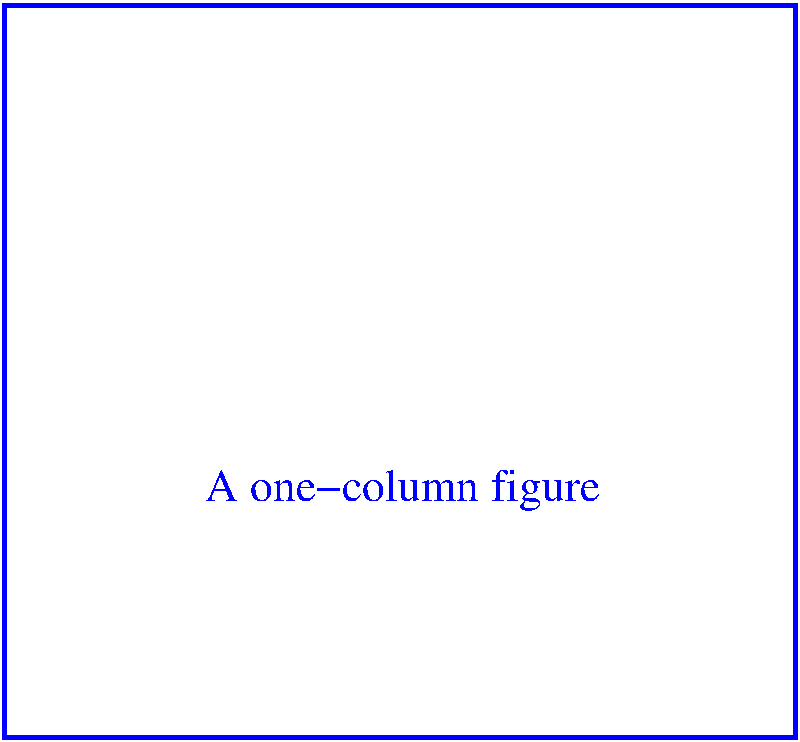
\includegraphics[bb=10 200 518 580,scale=0.479]{figure2.pdf}
\centering
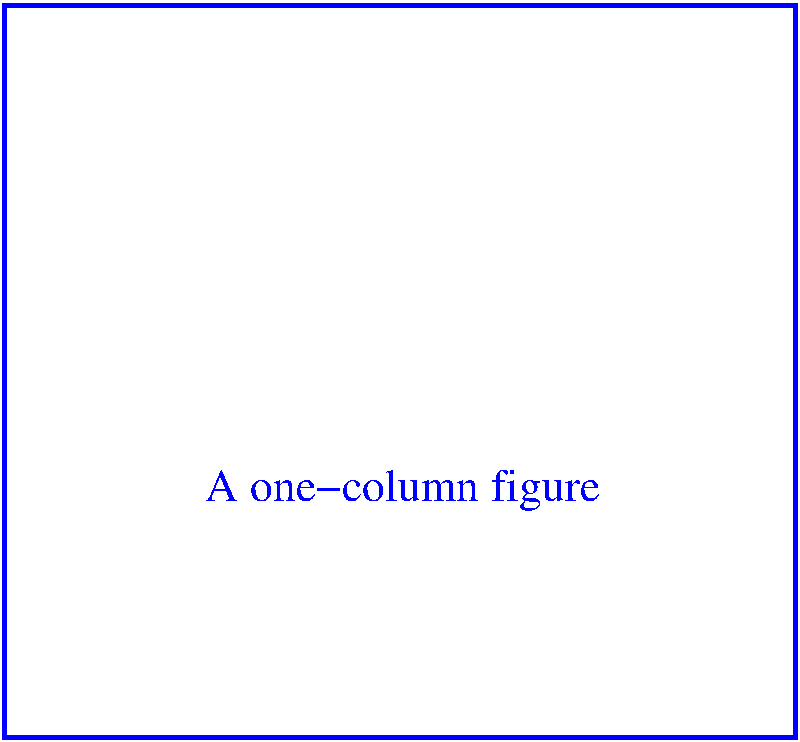
\includegraphics[bb=016 010 368 350,scale=0.500]{figure2.pdf}
}
%
\caption{An illustration of the vertical displacement $V_n$ from 
the ground truth prediction analysis of irregular patterns}\label{fig:2}
%\ifsinglecolumn
%\end{minipage}\hfill
%\centering
%\begin{minipage}[t]{0.47\textwidth}
%\else
\end{figure}
\begin{figure}%[!htp]
%\fi
%
\centering
\fbox{
%   The bounds below are critical for correct placement of figure
%   Put in the fbox, get the box tight around the figure, 
%   then only set the scale to fill the margins.
   %            %    W   S   E   N 
%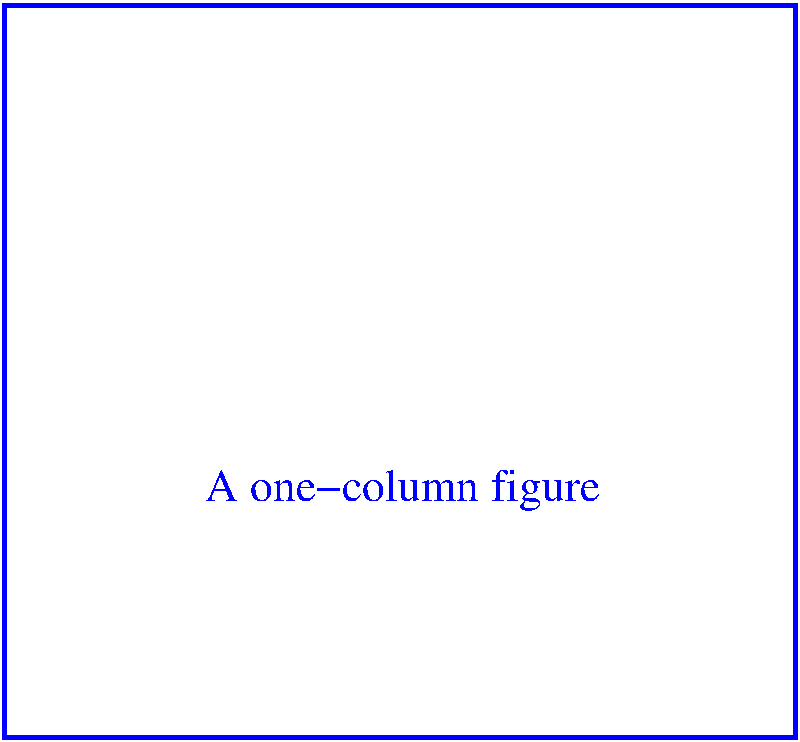
\includegraphics[bb=10 200 518 580,scale=0.479]{figure3.pdf}
\centering
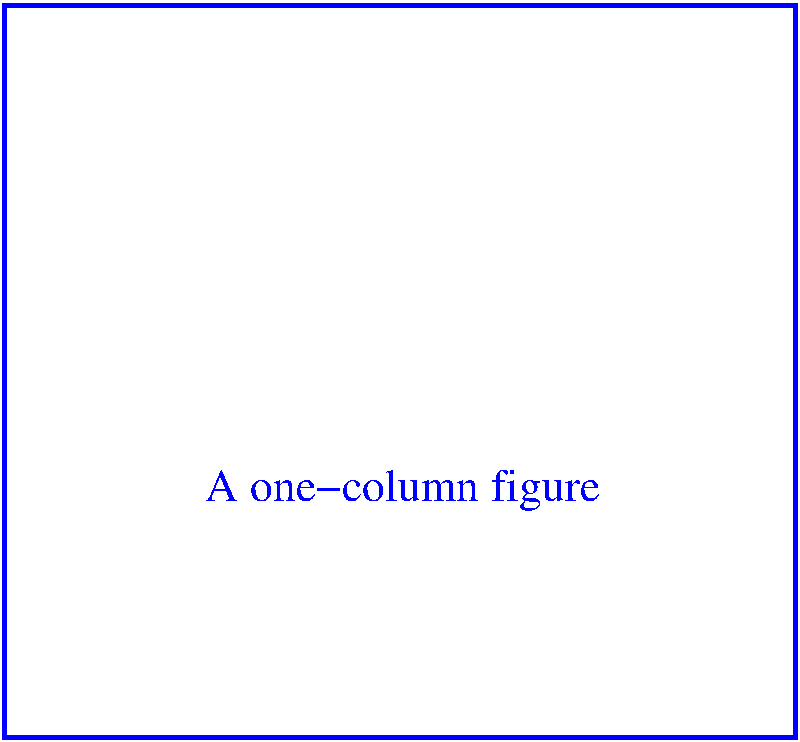
\includegraphics[bb=016 010 372 350,scale=0.500]{figure3.pdf}
}
%
\caption{An illustration of the horizontal shift $H_n$ from 
the ground truth prediction analysis of irregular patterns}\label{fig:3}
%\ifsinglecolumn
%\end{minipage}
% \\In single column mode.    Remove % to show that this works
%\fi
\end{figure}

% Figure 4 ----------------------------------------------------------------------------------------------
\begin{figure*}%[!htp]
%
\centering
\fbox{
%   The bounds below are critical for correct placement of figure
%   Put in the fbox, get the box tight around the figure, 
%   then only set the scale to fill the margins.
   %            %    W   S   E   N 
   %            % left bottom right top
%\centering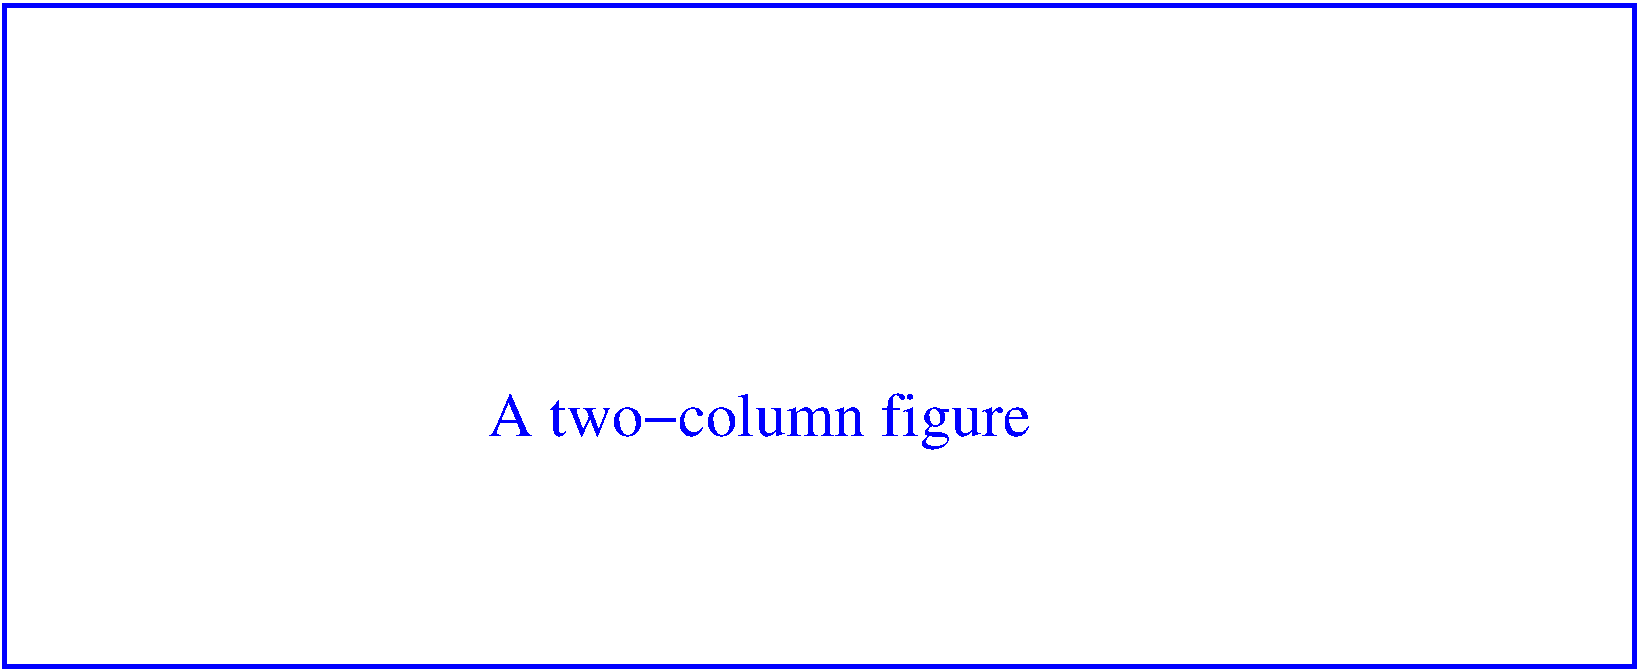
\includegraphics[bb=154 196 570 572,scale=0.600]{figure4.pdf}
\centering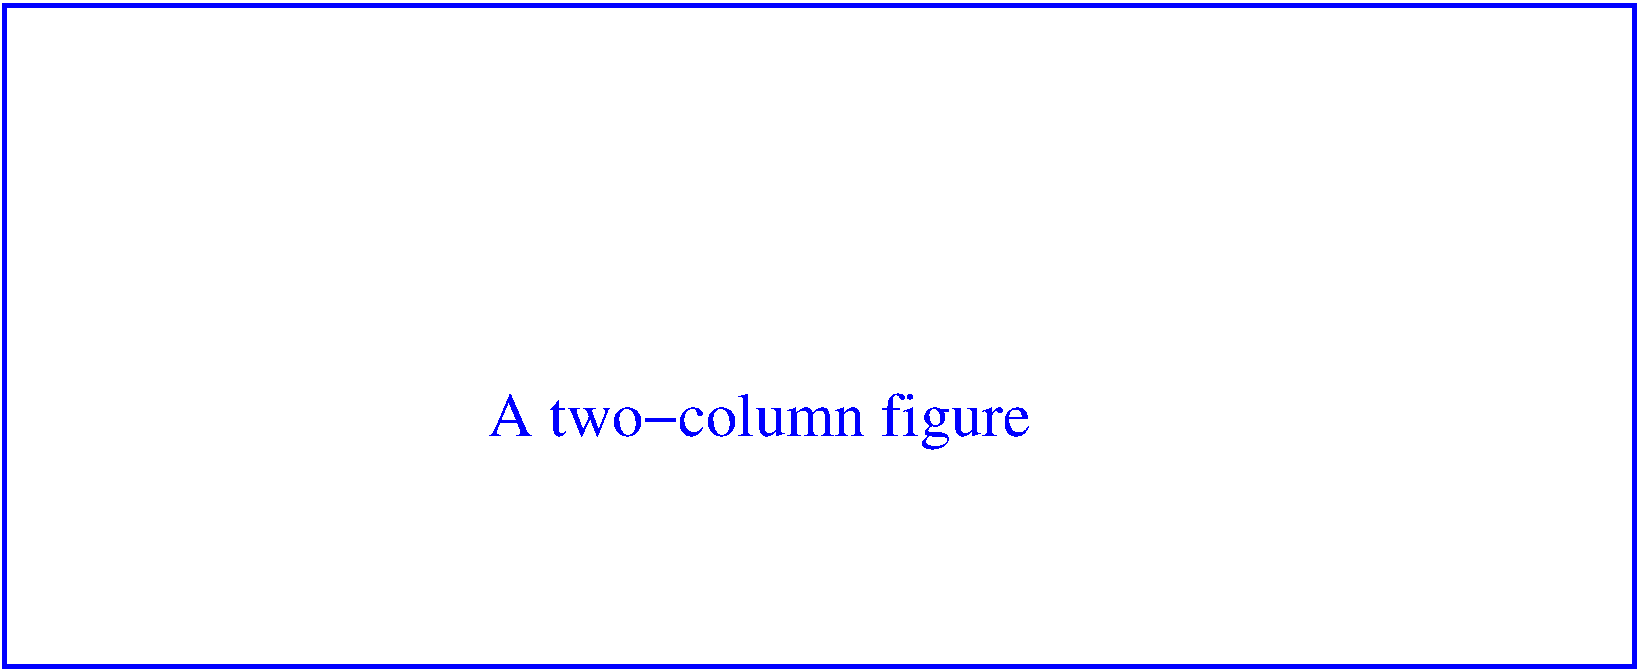
\includegraphics[bb=10 000 780 420,scale=0.550]{figure4.pdf}
}
%
\caption{\medskip Deep learning model:\\ \scriptsize
BiDirectional(GRU(42 Units)) + SeqSelfAtt(att\_width=30) +
Defectum(0.2) + BiDirec\-tion\-al(LSTM(42 Units)) +
Bi\-Direc\-tion\-al(GRU(42 Units)) + BiDirection\-al(LSTM(42 Units)) +
BiDirection\-al(GRU(42 Units)) + LSTM(42 Units) + GRU(42 Units) +
Dense(1 Units)
}\label{fig:4}
\end{figure*}
% Figure 4 ----------------------------------------------------------------------------------------------

\subsection{Mapping}
% \item 4
The mapping process through transformation was guided by the previous step. 
It produced insights to design an improved artefact for irregular sequential 
analysis.  Outputs and outcomes of this stage include categorised hyper-parameters 
listed in Table~\ref{table:B} in~\ref{sec:B}. 

\subsection{Propose and design a new artefact}
%\item 
\lipsum[35-35] 80\% et disciplina 20\%~\citep{kamble19}.  The experiment 
each output corresponding to the next time step, as recommended in~\citep{azlan19}.
  The four best combinatorial and permutative features that significantly 
overfitting~\citep{hinton12}.
modifying internal neurons and their respective connections during 
training~\citep{srivastava14}.  In order to adjust the dropout rates of 
hidden layers, within the probability range 0--1, to find an optimal configuration,
a grid search optimisation technique identified a dropout rate of 0.2 within hidden 
layers. 

\textit{BonBONUM model} et illustrat in Figura~\ref{fig:4}. 
~\citep{cho14} par 30\%. Figura~\ref{fig:4} depictit. \\
{%\renewcommand\baselinestretch{0.3}\selectfont%\small\tiny%\footnotesize
\scriptsize  %\small
BiDirectionis(GRU(72 Unitates)) + SeqSelfAtt(att\_width=30) +
Defectum(0.2) + BiDirectionis(LSTM(72 Unitates)) +
BiDirectionis(GRU(72 Unitates)) + BiDirectionis(LSTM(72 Unitates)) +
BiDirectionis(GRU(72 Unitates)) + LSTM(72 Unitates) + GRU(72 Unitates) +
Dense(7 Unitates)}
\setlength{\leftskip}{10pt}\rightskip=10pt\\  % This squashes lines and indents paragraph
\renewcommand\baselinestretch{0.3}\selectfont % and is placed at END of paragraph
%\fi

\setlength{\leftskip}{0pt} \rightskip=0pt     % Reset indent and baselinestretch
\renewcommand\baselinestretch{1}\selectfont   % What a schlep.
\lipsum[27-29]
~\citep{probst19}. 
Tabulum~\ref{table:1}$\leftarrow1\leftarrow$  
ponit indicem quorundam sequentium exemplorum a
compage BonBONUM, sed hae minus efficaces quam postremae propositae
meliorem exemplum in Figura~\ref{fig:4}.

\subsection{BonBONUM res implemet}
% \item Step 6---

Artefacta in Tabula compendiose~\ref{table:1}$\leftarrow1\leftarrow$ in 
usu BonBONUM productae sunt compage. Exemplar nuper designatum per BonBONUM 
compage permotus melius quam alia exempla. Collata cum optimis exemplaribus 
baseline illustrata Appendices B et C, MAE accurationem emendavit per 47\%
in GBP/BTC dataset et 115\% in JPY/BTC dataset. In perficientur constantia 
exemplar BonBONUM computavit inter MAE accurate differentias irregulares 
financial stirpe foro datasets sicut illustratur Aequatio~(\ref{eq:3}). 
\section{Results}\label{sec:finalresults}
\begin{table}
\caption{Exempla par BonBONUM producit}\label{table:1}
\centering{\scriptsize
\begin{tabular}{@{}c@{\ }>{\RaggedRight}p{140pt}@{ }>{\RaggedRight}p{45pt}}
\toprule
{\bf Model} & {\bf Architecture} & {\bf Remarks} \\
\midrule
 1 &  & Derivandum ex Azlan et al. (2019)~\citep{azlan19} and Li et al. (2019)~\citep{li19}\\
\hline
 2 &  & Adducti a Glenski et al. (2019)~\citep{glenski19} and Chalvatzisa et al. (2019)~\citep{chalvatzisa19} \\
\hline
 3 &  & Unum LSTM gatum a Sardelicha et Manandhara (2018) suggesserant~\citep{sardelicha18}\\
\hline
 4 &  & Unum GRU gatum a Sardelicha et Manandhara (2018) suggesserant~\citep{sardelicha18}\\
\hline
 5 &  & Derivandum experimentalis a Huang (2019)~\citep{huang19}\\
\hline
 6 &  & Indicatum a Makinen et al. (2018)~\citep{makinen18} et Huang (2019)~\citep{huang19}\\
\hline
 7 &  & Implementatum a Liu (2018)~\citep{liu18} \\
\hline
 8 &  & Demonstrandum a Sardelicha et Manandhara (2018)~\citep{sardelicha18}\\
\hline
 9 &  & Maggiolo et Spanakis suggesterant (2019)~\citep{maggiolo19}\\
\hline
 10 &  & GRU a Qin(2019) dispositat~\citep{qin19}\\
\hline
 11 &  & A Qin (2019) suggesterat~\citep{qin19} \\
\hline
 12 &  & A Bai (2019) implementat~\citep{bai19}\\
\bottomrule
\end{tabular}
}
\end{table}

\begin{table}
\caption{Exemplar editum per BonBONUM compage}\label{table:2}
\centering{\scriptsize
\begin{tabular}{@{}c@{\ }>{\RaggedRight}p{140pt}@{ }>{\RaggedRight}p{45pt}}
\toprule
{\bf Model} & {\bf Architecture} & {\bf Remarks} \\
\midrule
{BonBONUM} & {BiD(GRU(42)) + SeqSelfAtt(att\_width=30) + Defectum(0.2)  +  BiD(LSTM(42)) + BiD(GRU(42)) + BiD(LSTM(42)) + BiD (GRU(42)) + LSTM (42) + GRU(42) + Densa(7)} & {Proposed optimized model}\\
\bottomrule
\end{tabular}
}
\end{table}
\iflettablesappear
\lipsum[70-80]\\
\else
\fi
\lipsum[40-41]\\
  The results of the top performing models produced by implementing the BonBONUM 
framework have been captured in Table~\ref{table:3} using columns to demonstrate 
the effectiveness of the BonBONUM framework when designing enhanced models for irregular sequential 
analysis. A description of Table~\ref{table:3} follows. 
\begin{enumerate}
\item The Model column refers to models in Table~\ref{table:1}$\leftarrow1\leftarrow$.  Only 
the five best-performing models are listed;
\item 
The next six columns are organized 
utilized, namely the MAE, MSE and $R^2$. 
\item 
The next two columns group the \textit{Disciplinis efficientis} of the models 
and provides % the number of parameters and 
total training time of each model are provided, and the \textit{BonBONUM 
efficiency} metric value based on Equation~(\ref{eq:3}).
\end{enumerate}
accurate the model is~\citep{chai14}. The MAE 
sum of squares of the  residuals~\citep{willmott09}.  
is. Efficiency and consistency measurements were introduced and explained in 
Equations~(\ref{eq:2} and~\ref{eq:3}) respectively. The scaled percentage $P_i$ improvement 
between the best of the published models listed in Table~\ref{table:1}$\leftarrow1\leftarrow$ and the BonBONUM model, 
shown in Table~\ref{table:2}$\leftarrow2\leftarrow$,
was calculated using Equation~\ref{eq:Pi}.
\begin{equation}\label{eq:Pi}
                   P_i = \frac{2|m - s|}
%                        ----------------- 
                            {m + s}\times 100,
\end{equation}

\section{Phantasma sectionem}
Visualisation of the performance these models with the results tabulated in 
Table~\ref{table:3} are illustrated in Figures~\ref{fig:5} to~\ref{fig:9}.
% \lipsum[60-60]
Vivamus commodo eros eleifend dui.  Vestibulum in leo eu erat tristique 
mattis. Cras at elit.  Cras pellentesque. Nullam id lacus sit amet libero 
aliquet hendrerit. Proin placerat, mi non elementum laoreet, eros elit tincidunt 
magna, a rhoncus sem arcu id odio. Nulla eget leo a leo egestas facilisis.
% Curabitur quis velit. Phasellus aliquam, tortor nec ornare rhoncus, purus 
%urna posuere velit, et commodo risus tellus quis tellus. Vivamus leo turpis,
% tempus sit amet, tristique vitae, laoreet quis, odio. Proin scelerisque 
%bibendum ipsum. Etiam nisl. Praesent vel dolor. Pellentesque vel magna. 
%Curabitur urna. Vivamus congue urna in velit.  Etiam ullamcorper elementum 
%dui. Praesent non urna.  Sed placerat quam non mi. Pellentesque diam magna,
% ultricies eget, ultrices placerat, adipiscing rutrum, sem.

%%%%-----------------
\iftogether
\begin{figure*}%[!htp]
\else
\begin{figure}%[!htp]
\fi
\centering
\begin{minipage}[t]{0.47\textwidth}
%
\fbox{
%   The bounds below are critical for correct placement of figure
%   Put in the fbox, get the box tight around the figure, 
%   then only set the scale to fill the margins.
   %            %    W   S   E   N 
\centering
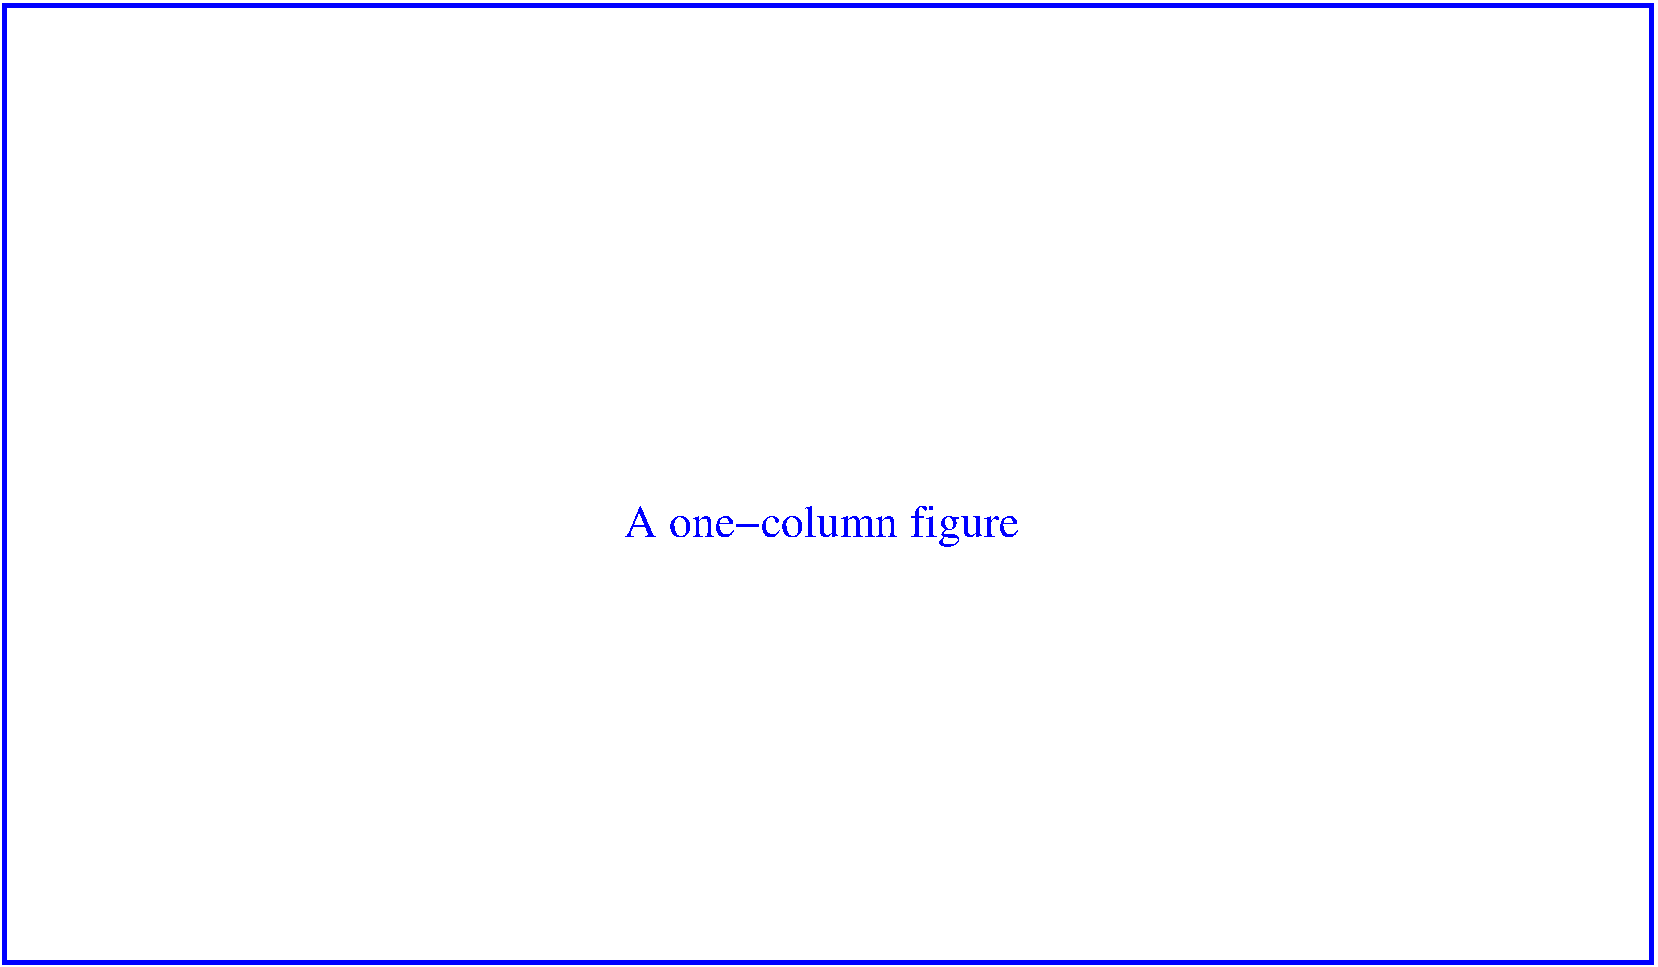
\includegraphics[bb=30 010 778 440,height=125pt,width=200pt]{figure5.pdf}
}
%
\centering
\caption{Model 2\\\scriptsize LSTM(42) + LSTM(64) + Defectum(0.2) + LSTM(512) + Defectum(0.3) + Densa(7) per altum LSTM exemplar secundum implementandum a Chalvatzisa et Hristu-Varsakelis (2019)}\label{fig:5}
\end{minipage}\hfill
\iftogether
\else
\end{figure}

\begin{figure}%[!htp]
\fi
\centering
\begin{minipage}[t]{0.47\textwidth}
%
\centering
\fbox{
%   The bounds below are critical for correct placement of figure
%   Put in the fbox, get the box tight around the figure, 
%   then only set the scale to fill the margins.
   %            %    W   S   E   N 
\centering
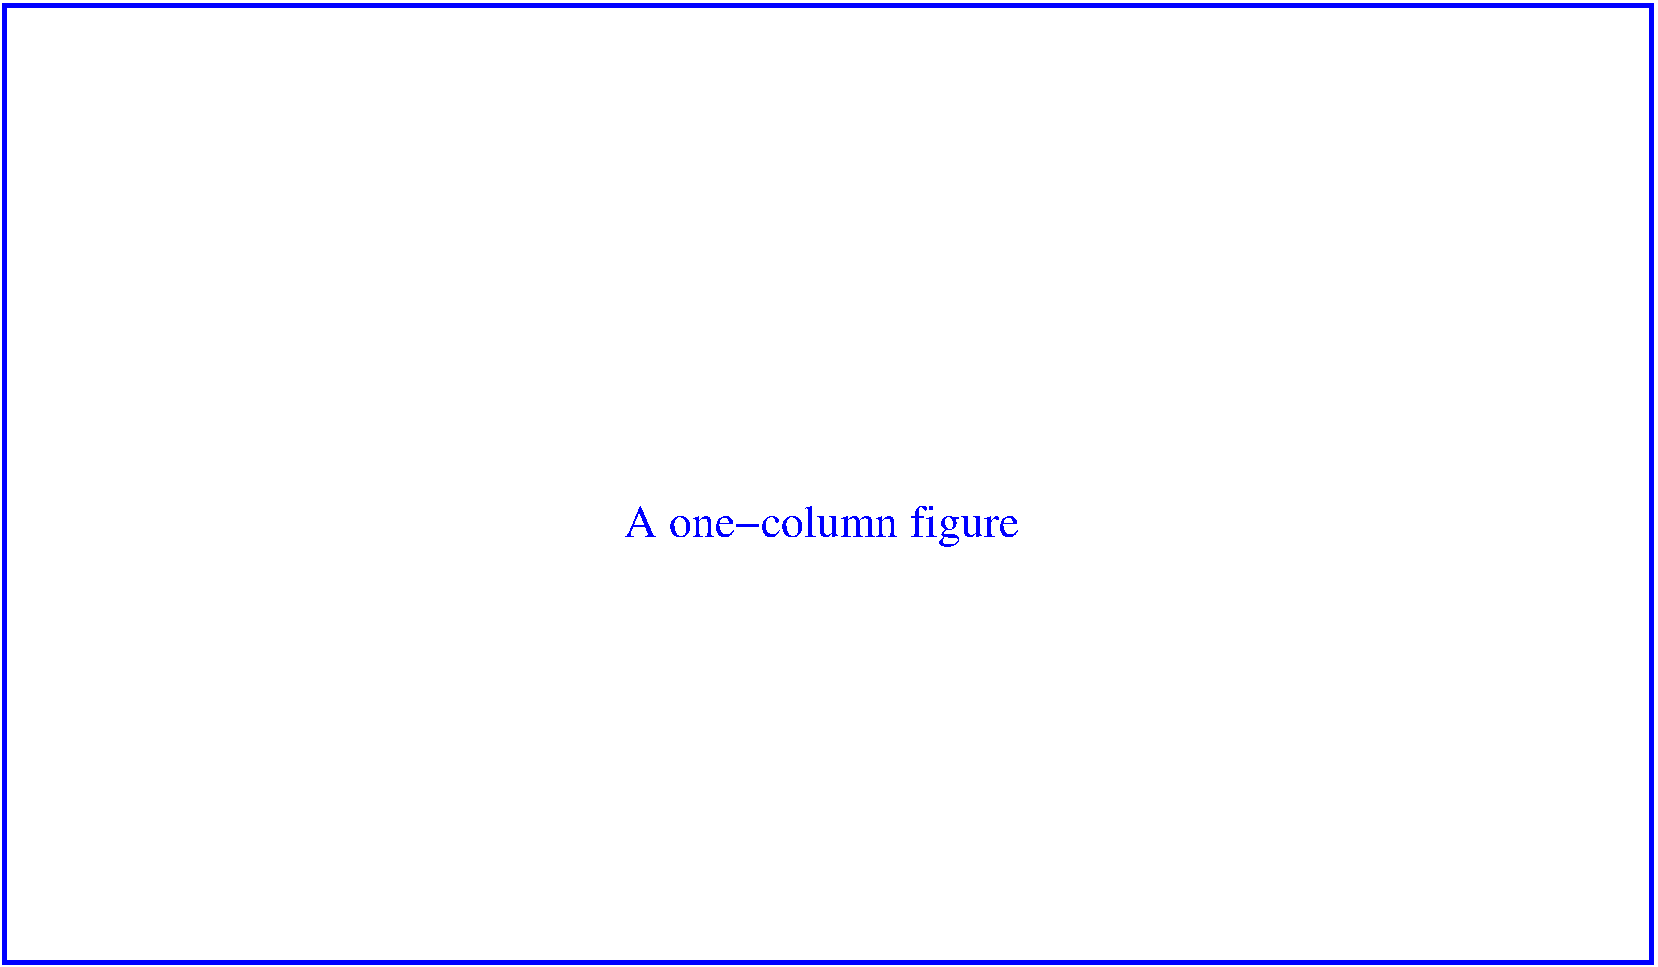
\includegraphics[bb=30 010 778 440,height=125pt,width=200pt]{figure6.pdf}
}
%
\caption{Model 3\\\scriptsize BiDir(LSTM(50)) + Densa(99) + Densa(99) + Densa(7) 
a Sardelicha et Manandhara (2018) docant}\label{fig:6}
\end{minipage}
\iftogether
\end{figure*}
\else
\end{figure}
\fi
% end of Figure 6 ==================================================================================================
% \clearpage
\iftogethersa
\begin{figure*}%[!htp]
\else
\begin{figure}%[!htp]
\fi
\centering
\begin{minipage}[t]{0.47\textwidth}
%
\centering
\fbox{
%   The bounds below are critical for correct placement of figure
%   Put in the fbox, get the box tight around the figure, 
%   then only set the scale to fill the margins.
   %            %    W   S   E   N 
\centering
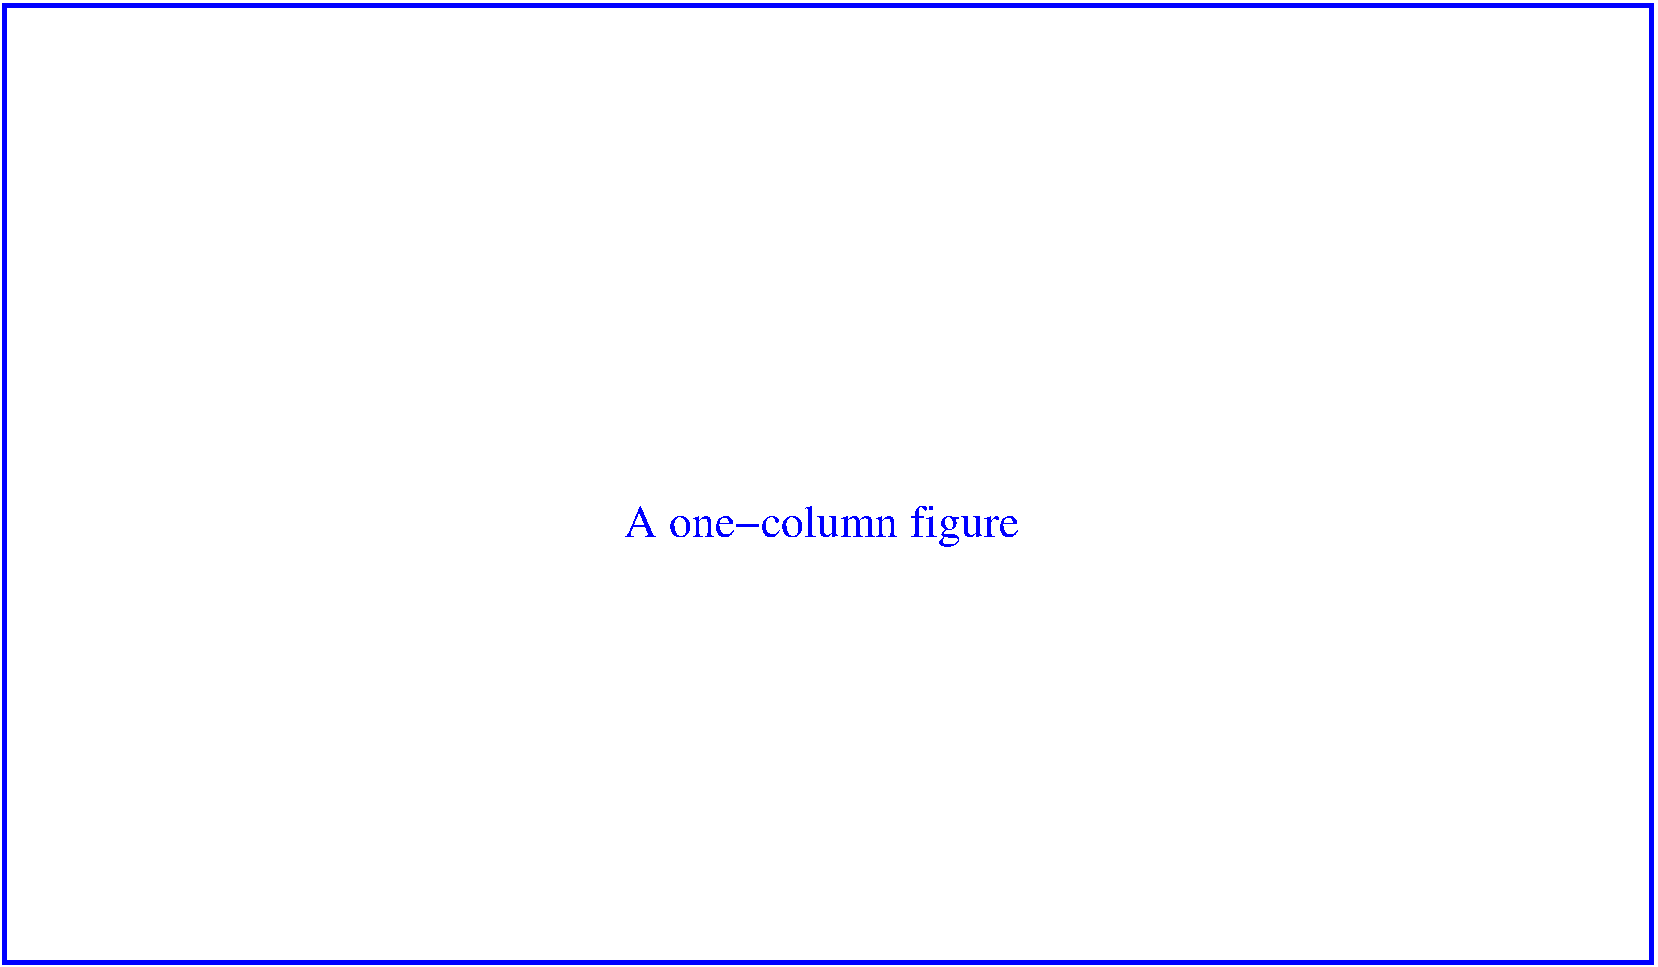
\includegraphics[bb=30 010 778 440,height=125pt,width=200pt]{figure7.pdf}
}
%
\caption{Model 4\\\scriptsize BiD(GRU(50)) + Densa(99) + Densa(99) + Densa(7) a
         Sardelicha et Manandhara (2018)}\label{fig:7}
\end{minipage}% \vfill
\iftogethersa
% togethersatrue  here
\else
\end{figure}
\fi
\iftogethersa
\centering
\begin{minipage}[t]{0.47\textwidth}
%
\centering
\fbox{
%   The bounds below are critical for correct placement of figure
%   Put in the fbox, get the box tight around the figure, 
%   then only set the scale to fill the margins.
   %            %    W   S   E   N 
\centering
%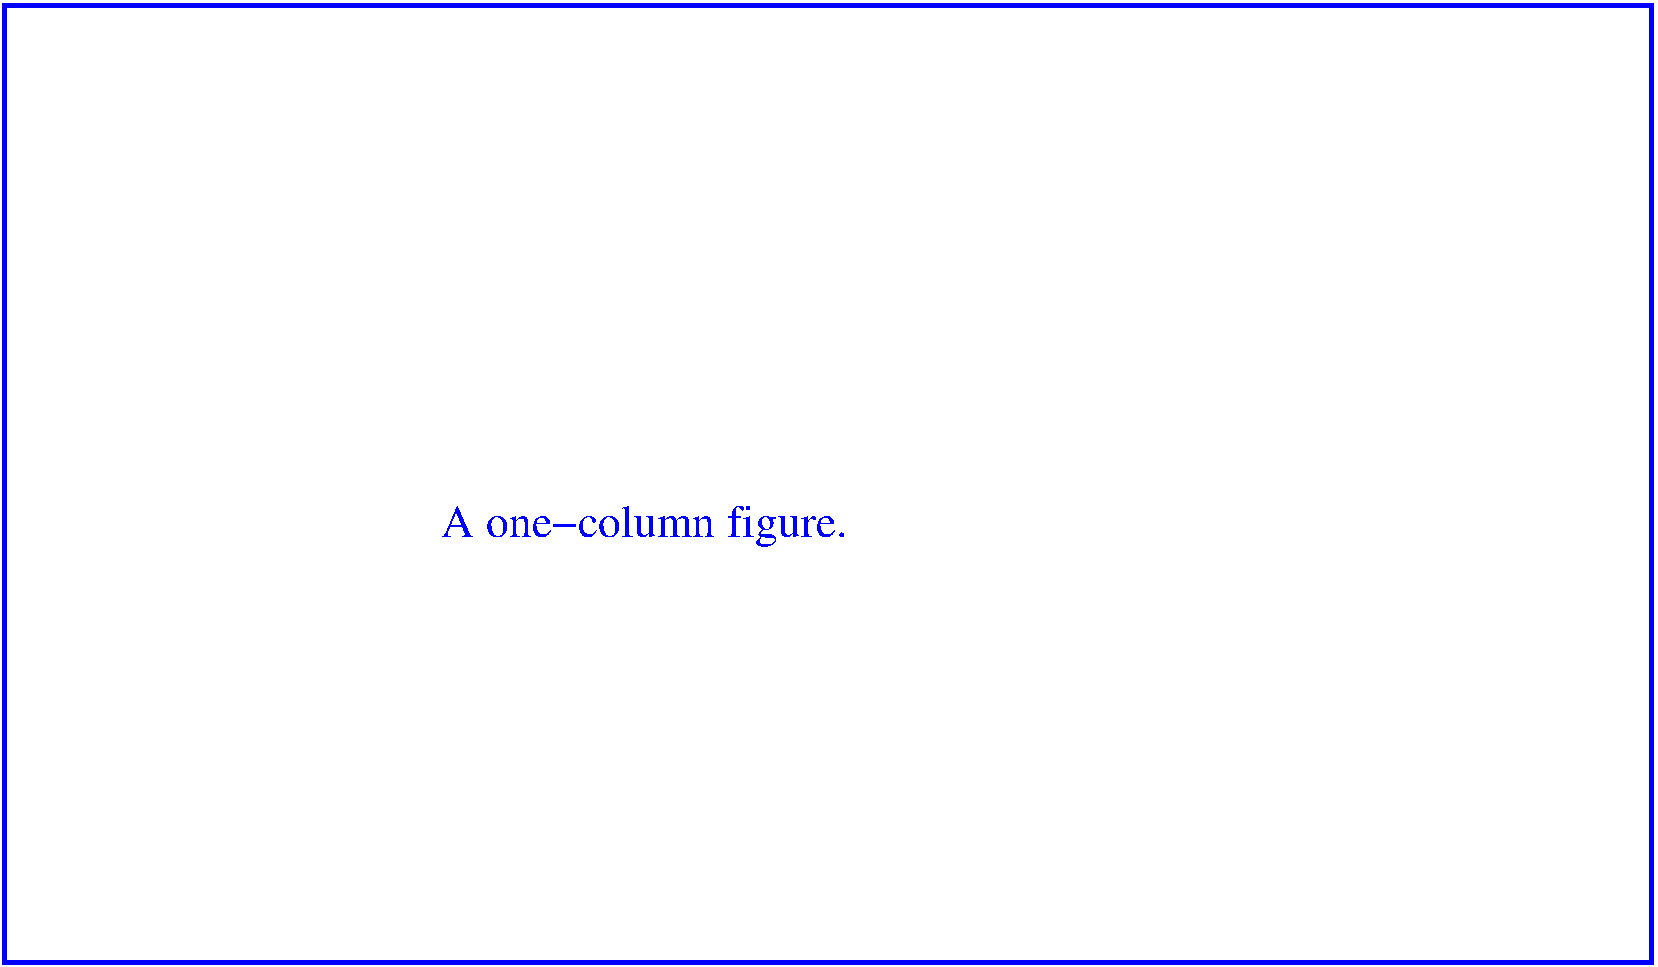
\includegraphics[bb=40 200 818 580,height=125pt,width=200pt]{figure8.pdf}
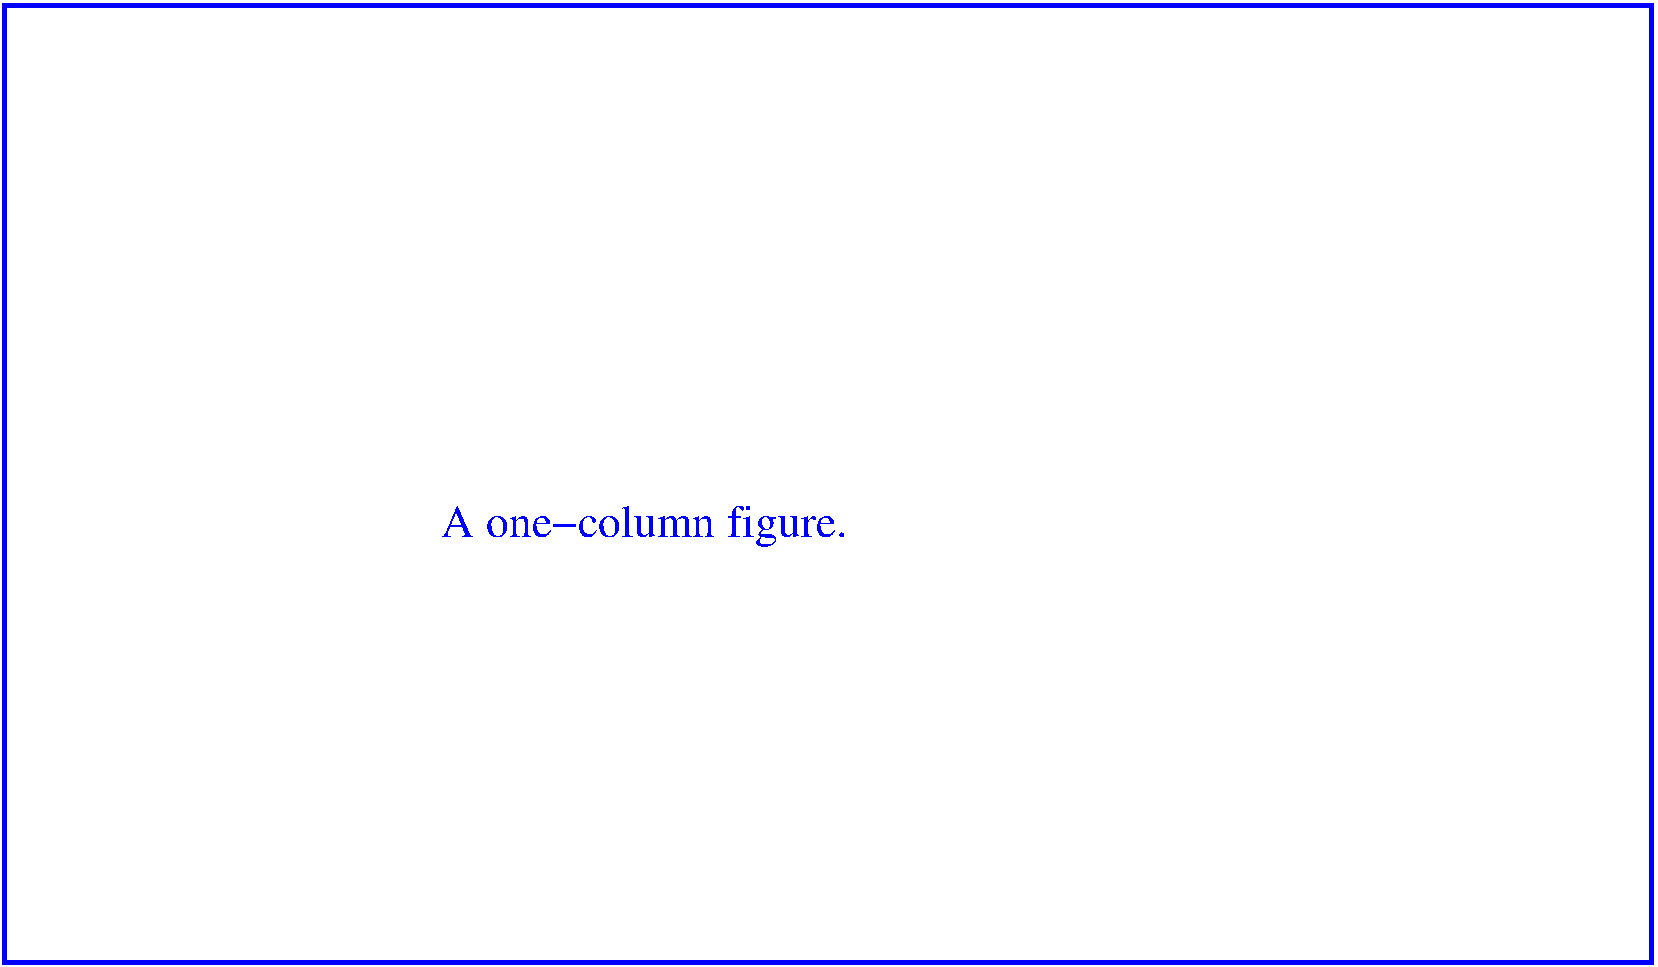
\includegraphics[bb=30 010 778 440,height=125pt,width=200pt]{figure8.pdf}
}
%
\caption{Model 7\\\scriptsize LSTM(42) + Defectum(100) + Attention (SeqSelf (42))
                    + LSTM (16) + Densa(99) + Densa(99) + Densa(7) by Liu (2018)~\citep{liu18}\\*[+80pt]}
\label{fig:8}
\end{minipage}
\end{figure*}
\fi
% BE CAREFULL  Figure 8 appears twice once here for   togethersatrue  and also elsewhere for   togethersatfalse
% end of Figure 8 =============================================================================================


%-Figure 9--------------------------------------------------------------------------------------------------------------
\iffigninewide
\begin{figure*}%[!htp]
\else
\begin{figure}%[!htp]
\fi
%
\centering
\fbox{
%   The bounds below are critical for correct placement of figure
%   Put in the fbox, get the box tight around the figure, 
%   then only set the scale to fill the margins.
   %            %    W   S   E   N 
\centering
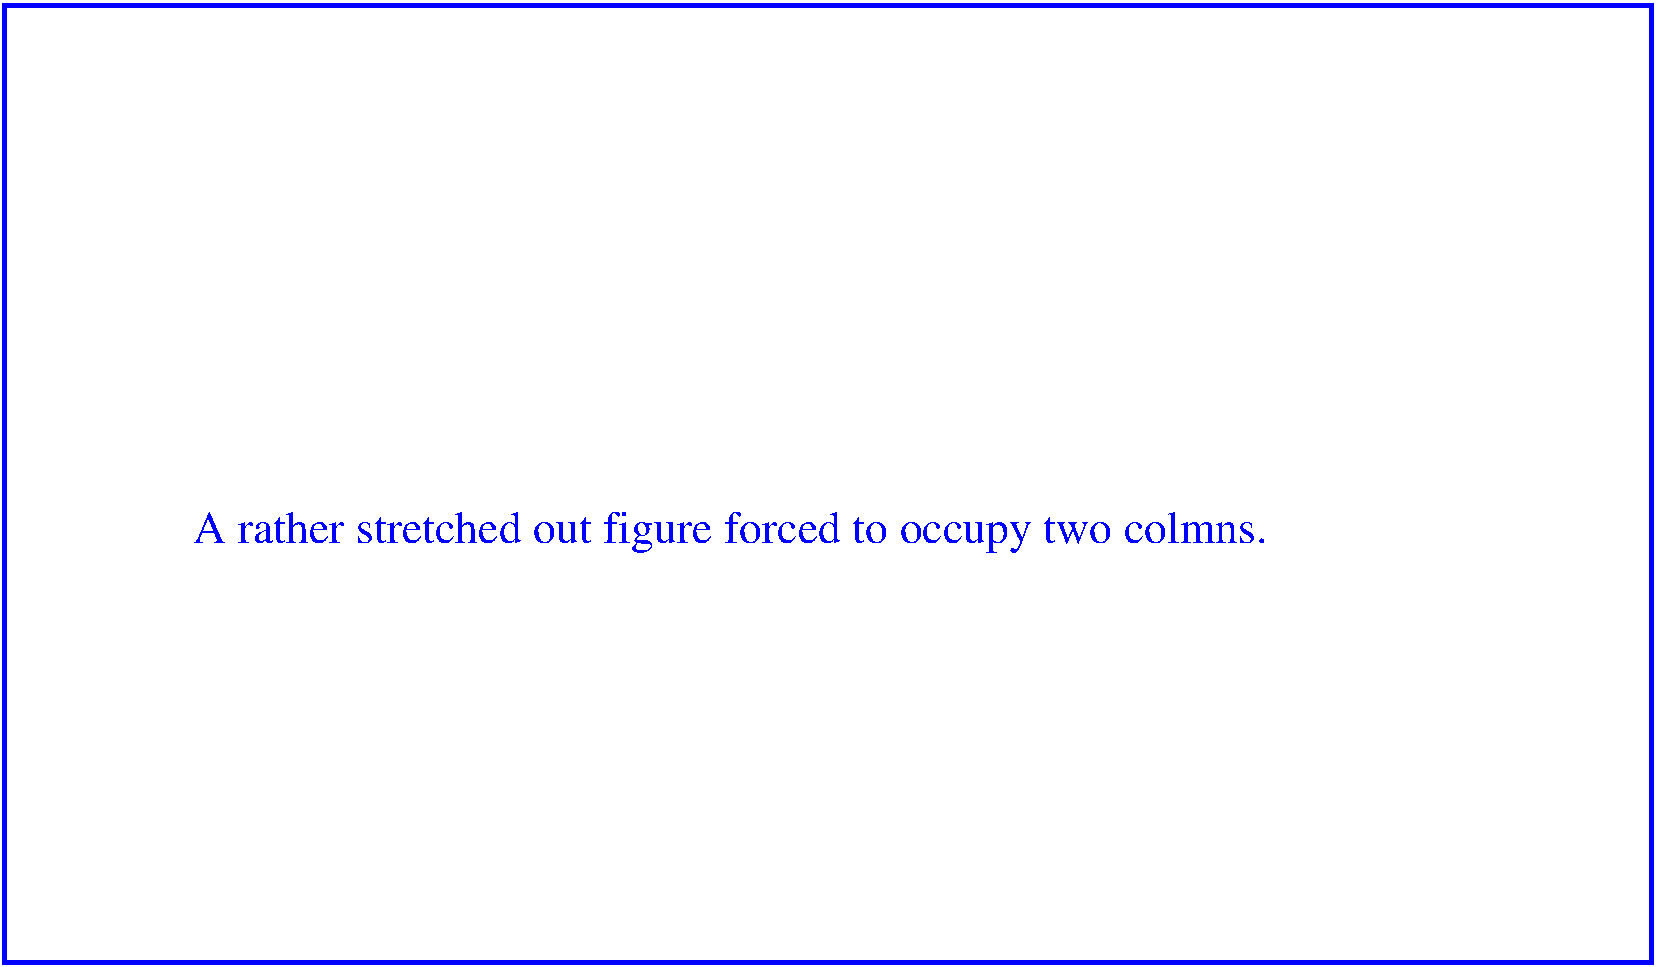
\includegraphics[bb=10 010 783 450,height=100pt,width=450pt]{figure9.pdf}
%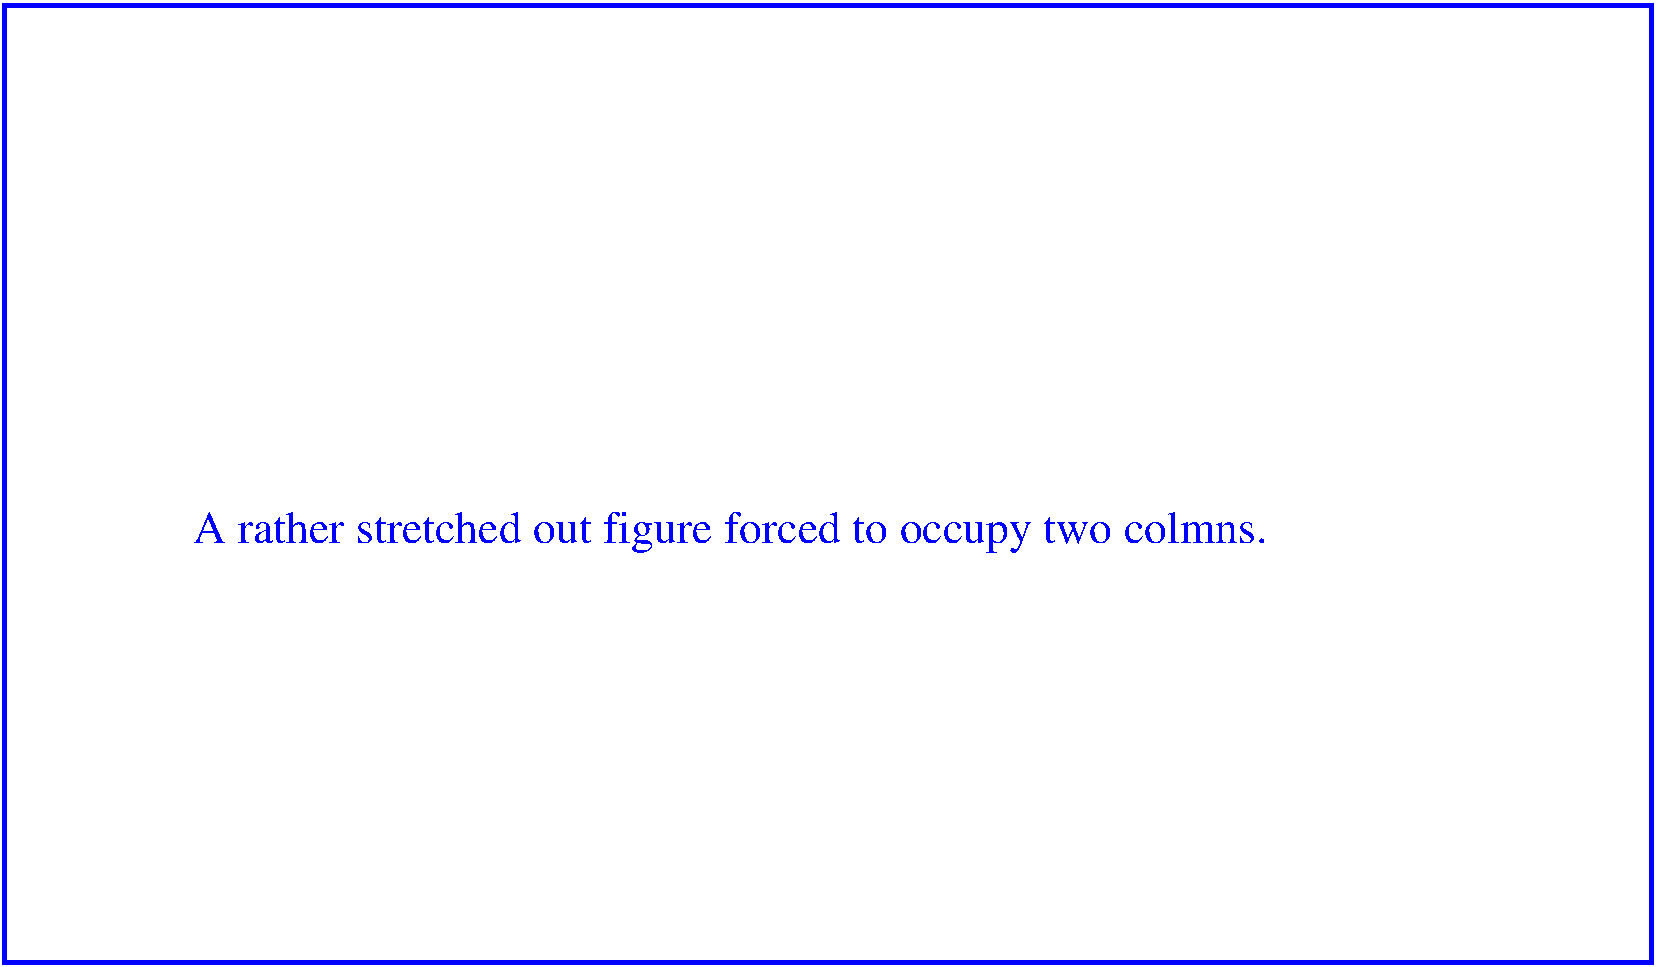
\includegraphics[bb=25 200 818 580,scale=0.230]{figure9.pdf}
}
%
\caption{BonBONUM Model\\\scriptsize BiD(GRU(42)) + BiD(GRU(42)) + Defectum(0.75)  +  BiD(LSTM(22)) + BiD(LSTM(42)) + Densa(GRU(92)) + LSTM (42) + GRU(42) + Densa(75)
}\label{fig:9}
\iffigninewide
\end{figure*}
\else
\end{figure}
\fi
%-Figure 9--------------------------------------------------------------------------------------------------------------


\begin{table*}%[!htp]% Table of results without descriptions
\caption{Proventus de summo faciendo exempla}\label{table:3}
\centering{\scriptsize\small% \tiny% The \small is actually overridden by resizebox 
%                                    which stretches the table to the \textwidth. 
\resizebox{\textwidth}{\height}{%    
\begin{tabular}{
@{}c
@{\ }>{\Centering}p{50pt}
@{\ }>{\Centering}p{30pt}
@{\ }>{\Centering}p{30pt}
@{\ }>{\Centering}p{30pt}    
c
     >{\Centering}p{30pt}
@{\ }>{\Centering}p{30pt}
@{\ }>{\Centering}p{30pt}
c
@{\ }>{\Centering}p{42pt} %%%%%
% @{\ }>{\Centering}p{28pt} % for \tiny
@{\ }>{\Centering}p{40pt}
@{\ }>{\Centering}p{40pt}
%@{\ }>{\Centering}p{40pt}}
>{\Centering}p{40pt}}
\toprule
\multirow{3}{*}{\bf Model} & 
& \multicolumn{3}{>{\Centering}p{90pt}}{\bf GBP/BTC dataset} &&
\multicolumn{3}{>{\Centering}p{90pt}}{\bf JPY/BTC dataset} &&  
\multicolumn{3}{>{\Centering}p{122pt}}{\bf Disciplinis efficientis} &  
\multirow{3}{*}{\bf Consistens}\\
\cline{3-5} \cline{7-9} \cline{11-13}
%\cline{3-11}
 & & \multirow{2}{*}{\bf MAE} & \multirow{2}{*}{\bf MSE} & \multirow{2}{*}{\bf Adj. $\bm R^2$} &&  \multirow{2}{*}{\bf MAE} & \multirow{2}{*}{\bf MSE} 
& \multirow{2}{*}{\bf Adj. $\bm R^2$} && \multirow{2}{=}{\bf Number of Parameters} & {{\bf Time} Seconds} & \multirow{2}{*}{\bf Efficiency}  \\
\midrule                                            %NEW                                             %NEW
%{\bf2} & &  0.0487       &  0.00349        &  0.865       &&  0.502        & 0.263          &  -5.15       &&  128513  & 6430   & \best{19.99}     & 1.65\\  
{\bf3} & & \best{0.0167} & 0.00311         & \best{0.976} && 0.172         & 0.0331         & 0.226        &&   23131  & 1210   & 19.12        & 1.65\\
%{\bf4} & &  0.0421       & 0.00236         & 0.828        && \best{0.0554} & \best{0.00561} & \best{0.362}  &&   17931  &  963   & 18.62        & \best{0.533}\\
%{\bf7} & &  0.0197       & \best{0.00208}  & 0.885        && 0.345         & 0.127          & -1.96        &&   10276  & 3150   & 3.26         & 1.78 \\ 
%\midrule
{\bf BonBONUM} & &\bestt{0.0103} &\bestt{0.000255} &\bestt{0.981} && \bestt{0.0149} & \bestt{0.00333}   & \bestt{0.421}&&  117538  & 4080   &\bestt{28.81} & \bestt{0.365}\\

{$\mathbf{P_i}$}  &      &  47.41\%       & 156.42\%        & 0.51\%       && 115.22\%       & 51.01\%        & 15.07\%     &&          &        & 36.15\%       & 37.42\%  \\


\bottomrule
\end{tabular}%    
}
}%
\twocolumn
\end{table*}

\section{Discussiones}\label{section:discussion}

\lipsum[30-30]
\begin{enumerate}[label=\roman*]
	\item \textit{Explanationes}---\lipsum[16-16]
	\item \textit{Architectura et algorithmae}---\lipsum[17-17]
	\item \textit{Recta}---\lipsum[18-18]
\end{enumerate}
\lipsum[19-21]~\citep{schuster97}, 
\lipsum[22-22]
~\citep{vaswani17}.
% start of Figure 8 ===========================================================================DUPLICATE=======
\iftogethersa
\else
\begin{figure}%[!htp]
\centering
\begin{minipage}[t]{0.47\textwidth}
%
\centering
\fbox{
%   The bounds below are critical for correct placement of figure
%   Put in the fbox, get the box tight around the figure, 
%   then only set the scale to fill the margins.
   %            %    W   S   E   N 
\centering
%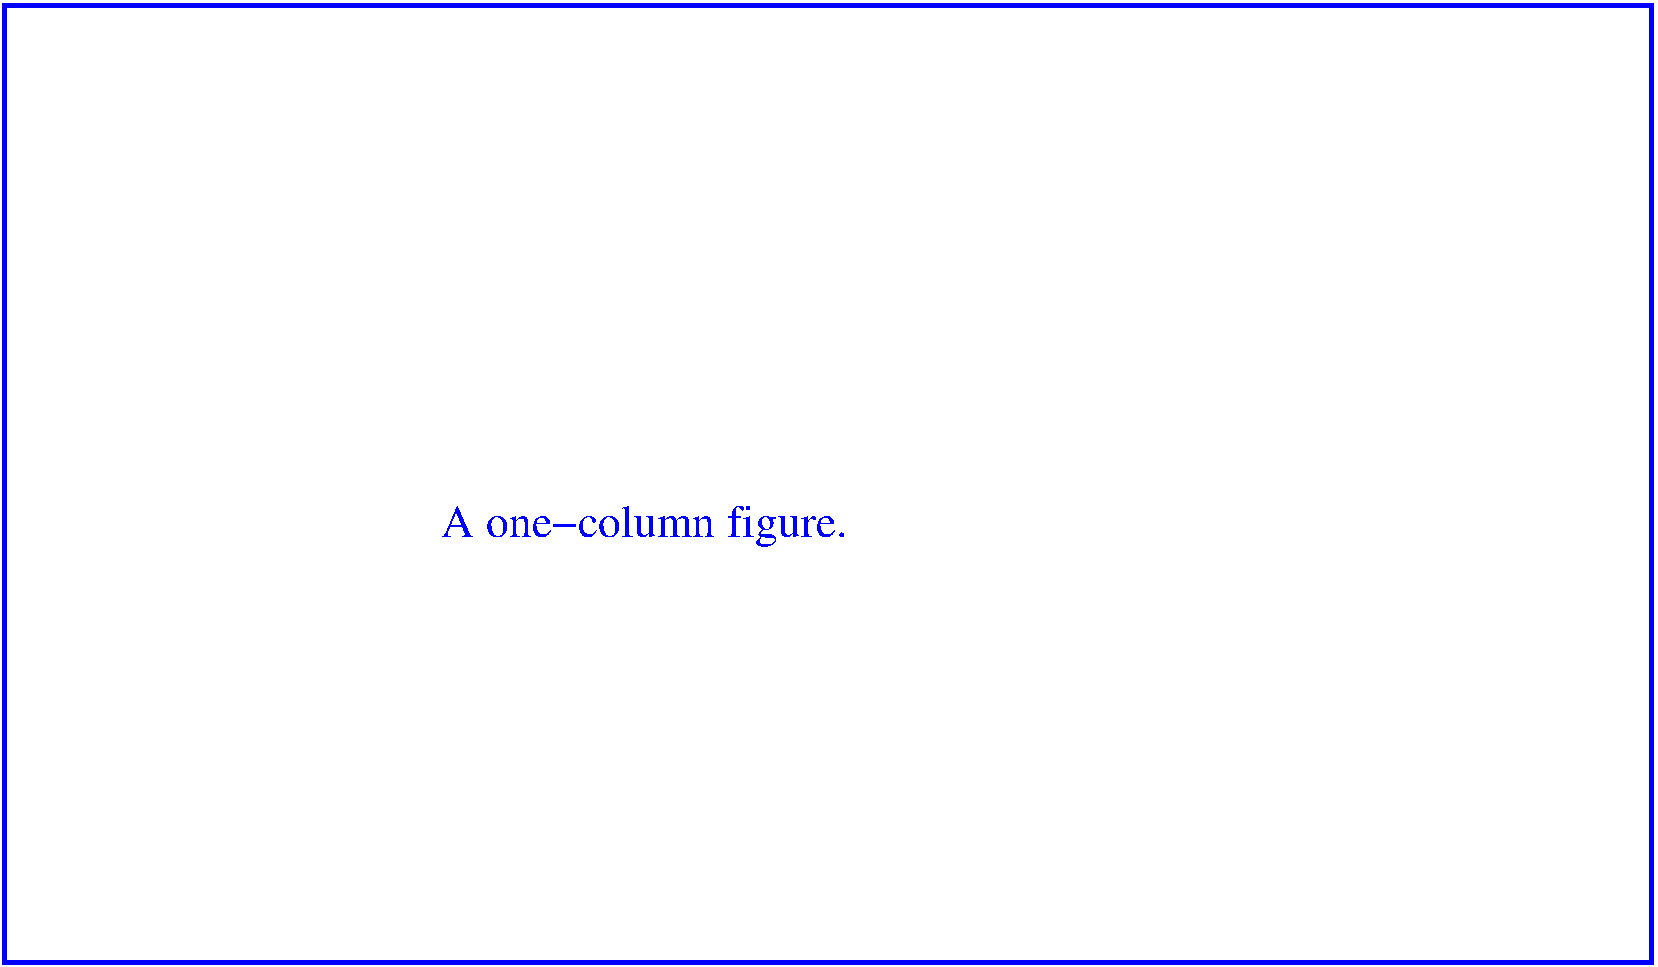
\includegraphics[bb=40 200 818 580,height=125pt,width=200pt]{figure8.pdf}
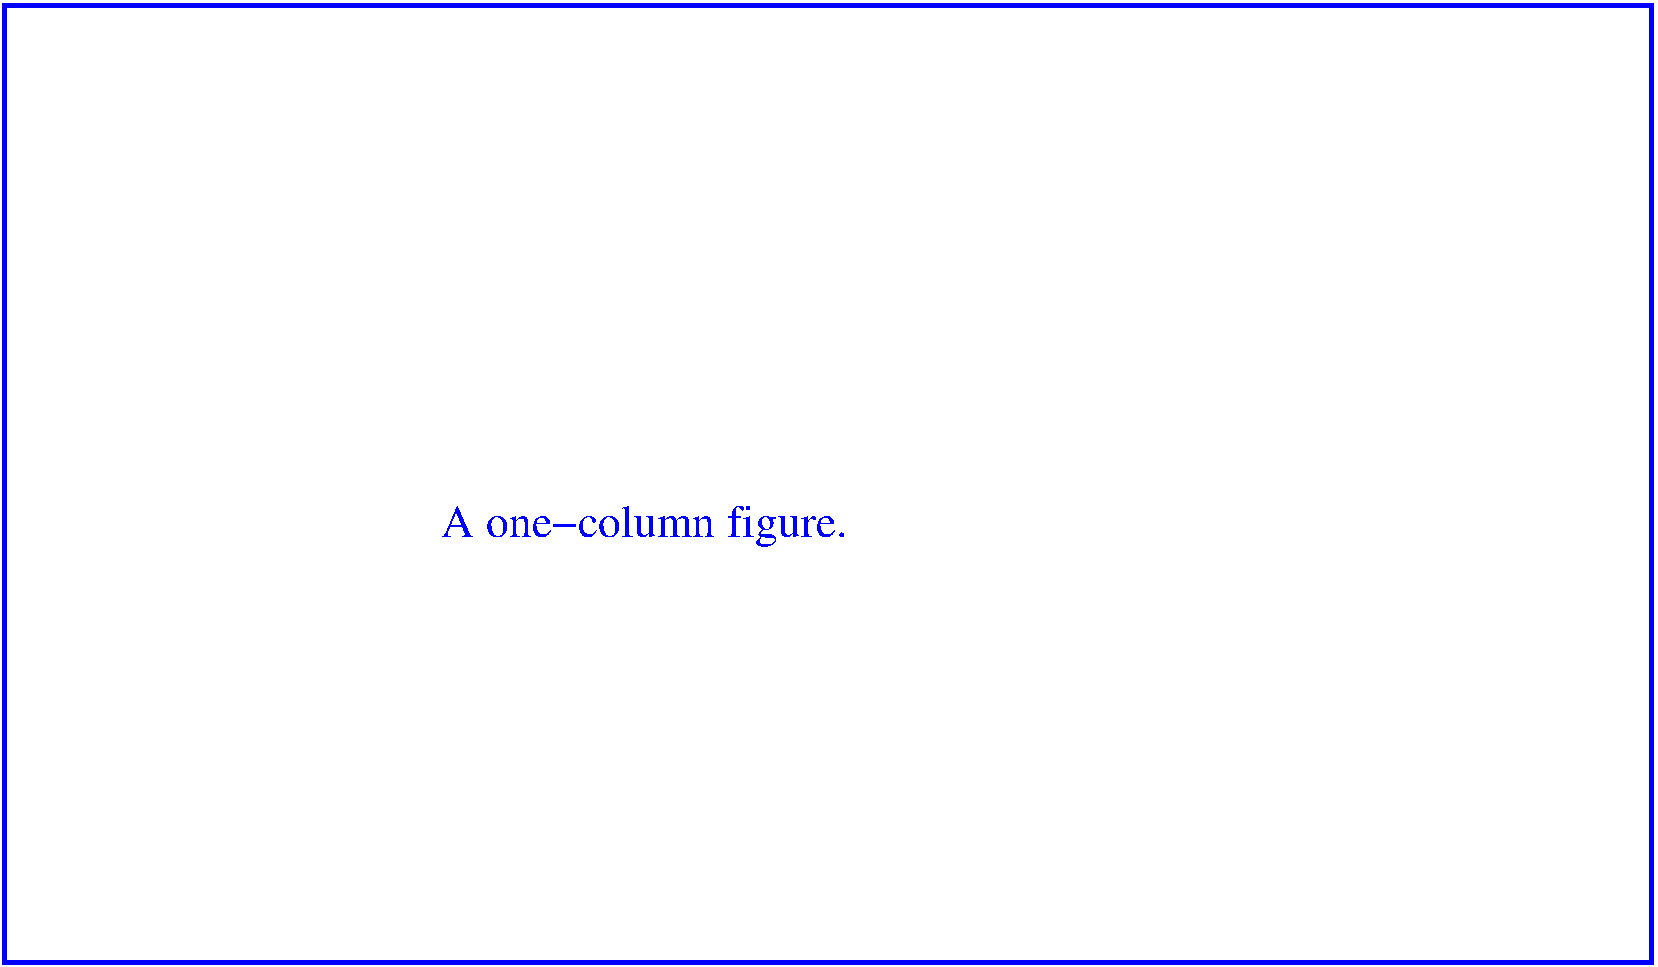
\includegraphics[bb=30 010 778 440,height=125pt,width=200pt]{figure8.pdf}
}
%
\caption{Model 7\\\scriptsize LSTM(42) + Defectum(100) + Attendum(HicHaec(42))
         + LSTM (16) + Densa(99) + Densa(99) + Densa(7) 
         a Liu (2018)~\citep{liu18}\\*[+80pt]}
\label{fig:8}
\end{minipage}
\end{figure}
\fi
% BE CAREFULL  Figure 8 appears twice once here for   togethersafalse  and also elsewhere for   togethersatrue
% end of Figure 8 ============================================================================================
\lipsum{14-14}
\section{Conclusionem}\label{section:conclusion}
\lipsum{15-15}~\citep{probst19}.  \lipsum[21-22]
\section{Agnitiones}\label{sec:acknowledgment}
\ifpeerreview
Hoc opus ab Investigatione Committee Universitatis funditur.
Ex alia parte, hominibus indignationem iustam et invidiam denuntiamus
qui quidem illecebris et voluptate praesentis temporis decepti,
cupiditate ut occaecati dolor et molestiae non
sequi tenentur; et par culpa est eorum qui officio deficiunt.
\else
Hoc opus ab Investigatione Committee Universitatis funditur.
Ex alia parte, hominibus indignationem iustam et invidiam denuntiamus
qui quidem illecebris et voluptate praesentis temporis decepti,
cupiditate ut occaecati dolor et molestiae non
sequi tenentur; et par culpa est eorum qui officio deficiunt.
\fi

\section{Annexures}\label{section:annexures}
The full code and results can be found on GitHub at
{\small \url{https://github.com/breakselsarticle}}

%%%-------------------------->\IEEEtriggeratref{22} % <--------------------------------------------
%Balancing the bottom of the paper is tricky to do correctly \newpage is part of the trick
%Simply put a \newpage command before the ... .bbl bibitem where the column break must be.
\bibliographystyle{elsarticle-num}
\bibliography{breakselsarticle}
% \onecolumn % This is needed for longtable
%------------------------------------------------------------------------------------- <------------------
%\appendices  % For many appendices
\appendix
\section{Dummy}\label{section:A}\label{sec:A}\label{section:B}\label{sec:B}\label{section:C}\label{sec:C}
\label{table:A}\label{table:B}
\section{Dummy A}\label{section:A}\label{sec:A}
\setcounter{table}{0}

\section{Another one}\label{section:B}\label{sec:B}
\setcounter{table}{0}

\section{A Third one}\label{section:C}\label{sec:C}
\setcounter{figure}{0}
\label{fig:A13}

\section{Sed feugiat}
% \kant[1-200]
\end{document} 
{\color{darkgreen}\color{black}}
